\chapter{Introduction}

\textbf{\textcolor{red}{THIS THESIS IS CURRENTLY AN UNPUBLISHED DRAFT. IT HAS
NOT BEEN SUBMITTED AND MAY HAVE MISSING CITATIONS AND CONTENT}}

Although nuclear structure has been studied since at least late 19th century, a
complete understanding of the proton's spin has eluded scientists.  Early models
of the proton structure such as the three valence quark model could accurately
predict the charge and spin of the proton, yet when measured in the late 1980's
this simplistic model was found to be wrong, in an event known as the`proton
spin crisis' (Figure~\ref{fig:spin_crisis_cartoon}). One of the challenges of
particle physics is to create a framework which can accurately describe matter,
as well as predict the behavior of matter at all energy scales. Protons and
neutrons are baryons which make up the majority of the mass in the visible
universe, yet fully understanding the origins of their properties--such as spin,
still eludes us. However, through the application of the scientific method over
many generations of physicists, we have magnificently described this important
particle, and understood many of its properties.  However, one property which
still defies our descriptions is its fundamental angular momentum, spin.
	
Our understanding of the proton has evolved and sharpened since the first
experiments in deep inelastic scattering showed that the proton is not a
fundamental particle~\cite{Breidenbach1969}. Gell-Mann later planted the seeds
of a theoretical framework which could in part describe some of the structure of
baryons, a class of hadrons which we may n{\"a}ively describe as composed of three
`valence quarks'~\cite{Bjorken1969}. We can apply well known sum rules to the
individual spins of the valence quarks which compose the proton in our naive
valence-model to produce a correct prediction for the proton's spin
${1}\over{2}$. When experimenters set out to measure the contribution of these
valence quarks in 1988 at the EMC experiment \cite{Ashman1988}, they were
surprised to find that the valence quarks carry only a small fraction of the
proton's spin, especially in light of the fact that in the three-quark model,
one can easily build a spin $1/2$ particle from three spin $1/2$ quarks. 

Although recent papers \cite{Povh2016} suggest that this `spin crisis'
(Figure~\ref{fig:spin_crisis_cartoon}) is simple due to mis-attribution of spin,
most literature to date has focused on understanding how to model the proton
with parton distribution functions. These parton distribution functions come in
many varieties, and probe different degrees of freedom within the proton, in
both the case of unpolarized parton distribution functions, and polarized parton
distribution functions. 

\begin{figure}
  \centering
  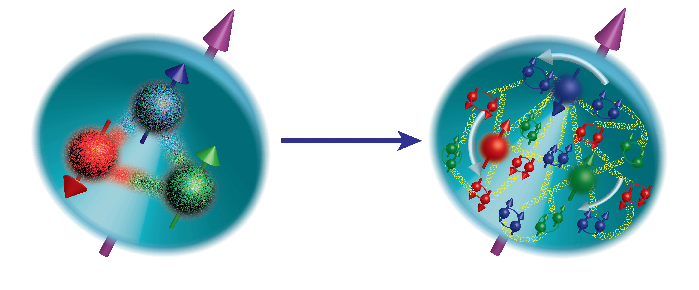
\includegraphics[width=0.8\linewidth]{./figures/figures_introduction_nucleon_picture.png}
  \caption{
    Left: the n{\"a}ive quark model, while predicting the correct spin of the
    proton, does not bear fruit when the quark spin contribution is measured.
    Right: a more realistic cartoon of the proton as a composite of gluons,
    valence quarks and sea-quarks~\cite{Accardi2012}.
  }
  \label{fig:spin_crisis_cartoon}
\end{figure}
 
\section{Scope and Objectives of This Work} 

In the first part of this thesis, I will describe the research I carried out
between May of 2010 through August of 2016.  This analysis comprises the body of
work devoted to calculating $A_L$ for the $W\rightarrow\mu$ decay. The results
of this analysis are used in global fits to constrain the total contribution of
quarks and anti-quarks in the so-called `proton-sea' to the proton's total spin.

In the second portion of this work, I will discuss the `Vernier Analysis', which
is instrumental for every single-cross-section calculation taken with RHIC data.
The thrust of the Vernier Analysis is to determine the beam luminosity at
PHENIX's interaction point. This enables one to normalize the results to the p+p
cross-section. This is done with a series of specialized Vernier-Scans, where
beams are scanned across one-another in order to measure beam geometry. The
luminosity can then be calculated from first principals, and compared to the
estimated machine luminosity published by RHIC's collider-accelerator
department. I produced an entire software framework for handling data cleaning,
analysis, visualization and simulation.
